\documentclass[a4paper, 11pt]{article}
\usepackage[italian]{babel}
\usepackage[utf8x]{inputenc}
\usepackage[T1]{fontenc}
\usepackage{graphicx}
\usepackage{longtable}
\usepackage{float}
\usepackage{wrapfig}
\usepackage{rotating}
\usepackage[normalem]{ulem}
\usepackage{amsmath}
\usepackage{calc}
\usepackage{lastpage} % Required to determine the last page for the footer
\usepackage{extramarks} % Required for headers and footers
\usepackage{textcomp}
\usepackage{marvosym}
\usepackage{wasysym}
\usepackage{amssymb}
\usepackage{hyperref}
\usepackage{enumitem}
\usepackage[a4paper]{geometry}
\usepackage[section]{placeins}
\usepackage{lmodern}
\usepackage{array}
\usepackage{subcaption}


%\geometry{hmargin=2.3cm}

\topmargin=-0.45in
\evensidemargin=0in
\oddsidemargin=0in
\textwidth=6.25in
\textheight=9in
\headsep=0.25in

\usepackage[normalem]{ulem} % [normalem] prevents the package from changing the default behavior of `\emph` to underline.
\usepackage{fancyhdr}
\usepackage{array}

\renewcommand{\baselinestretch}{1.1} 

\newcommand{\hmwkTitle}{Elaborato\ Ingegneria Del Software}

\pagestyle{fancy}
\lhead{\nouppercase{\leftmark}}
\rhead{\nouppercase{\rightmark}}
\chead{}
\lfoot{}
\cfoot{\thepage}
\rfoot{}
\renewcommand{\headrulewidth}{0.4pt}
\renewcommand{\footrulewidth}{0.4pt}


\def\changemargin#1#2{\list{}{\rightmargin#2\leftmargin#1}\item[]}
\let\endchangemargin=\endlist 

\newcolumntype{L}{>{\fontseries{l}\selectfont\arraybackslash}p{0.7\textwidth}}

\newcommand{\safeImage} [2] [\textwidth]{%
	\begin{figure}[H]
		\centering
	\IfFileExists{#2}{\includegraphics[width={#1},keepaspectratio]{#2}}{\includegraphics{example-image-a}}
	\end{figure}
}

\newcommand{\breakcell}[2][l]{\begin{tabular}[t]{@{}#1@{}}#2\end{tabular}}

\newcommand{\usecase}[5]{%
\begin{table}[H]
	%\vspace*{0.5 cm}
	\centering
	\renewcommand{\familydefault}{\ttdefault}\normalfont
\begin{tabular}{| >{\fontseries{b}\selectfont} p{0.2\textwidth} | L |}
	\hline
	ID&{#1}\\\hline
	Attori&{#2}\\\hline
	Precondizioni&{#3}\\\hline
	Sequenza&{#4}\\\hline
	Postcondizioni&{#5}\\\hline
\end{tabular}
\end{table}

}

\begin{document}

	\clearpage
%	\maketitle
\begin{titlepage}
	\centering
	\vspace*{\fill}
	
\includegraphics[width=0.15\textwidth]{logo.png}\par\vspace{1cm}
	{\scshape\LARGE Università degli Studi di Verona \par}
	\vspace{1cm}
	{\scshape\Large Ingegneria del Software\par}
	\vspace{1.5cm}
	\line(1,0){250} \\
	{\huge\bfseries Med-H\par}
	{\Large\bfseries Documentazione al prototipo\par}
	\line(1,0){250} \\
	\vspace{2cm}
	{\Large\itshape Mirko Morati, Noè Murr\par}
	\vspace{5cm}
	\vspace*{\fill}
	% Bottom of the page
	{\large \today\par}
\end{titlepage}
\thispagestyle{empty}
\newpage
\tableofcontents
\newpage

\section{Introduzione}
Obiettivo dell'elaborato è la progettazione di un prototipo software per la gestione della prescrizione di farmaci da parte dei medici di base di una regione.
In questa relazione ci proponiamo di raccogliere la documentazione sviluppata e di fornire spiegazioni e dettagli sulle scelte progettuali ed implementative. 

\section{Requisiti}
Di seguito viene riportato il testo dell'elaborato. I requisiti funzionali vengono identificati con una linea tratteggiata.

\begin{changemargin}{1cm}{0.5cm} 
Si vuole progettare un sistema informativo per gestire le prescrizioni di farmaci da parte dei medici di base di una regione. Il medico di base effettua la prescrizione di farmaci su richiesta del paziente (nel caso di farmaci legati a malattie croniche del paziente stesso) o in seguito alla visita. Nel caso di prescrizione su richiesta, il paziente può richiedere la prescrizione alla segreteria del medico che si occuperà di raccogliere le richieste, far preparare le ricette al medico e consegnare le prescrizioni ai pazienti.

\dashuline{I farmaci potranno essere prescritti anche da eventuali medici consorziati con il medico di base di riferimento o in caso di assenza del medico di base, dal medico sostituto designato}.
\dashuline{Ogni prescrizione è caratterizzata dall’indicazione del paziente a cui fa riferimento, dalla data di emissione, dalla data di scadenza, dai farmaci prescritti. Ogni prescrizione è dotata di un codice identificativo univoco}. La prescrizione deve essere presentata in farmacia per poter acquistare i farmaci necessari. Il farmacista utilizza la prescrizione, unitamente alla tessera sanitaria del paziente, per rilasciare lo scontrino parlante. In caso il medico abbia prescritto un farmaco e la farmacia non ne abbia a disposizione, il farmacista provvederà ad ordinare il farmaco per il paziente.
\dashuline{Per ogni paziente sono memorizzati: il codice sanitario univoco, il cognome, il nome, la data di nascita, il luogo di nascita, l’indirizzo di residenza (via, civico, cap, città, provincia). Per ogni paziente è possibile memorizzare gli eventuali fattori di rischio presenti (anche più d’uno)}.

\dashuline{Per ogni medico di base si registrano il codice fiscale, il codice univoco assegnato a livello regionale, il cognome, il nome, la data e il luogo di nascita. Per i medici di base con specializzazione si registrano anche l’ultima specializzazione ottenuta e la data di conseguimento. Ad ogni medico sono legate tutte le prescrizioni effettuate}.

\dashuline{Il medico può richiedere al sistema di visualizzare la lista dei farmaci prescritti ad un certo paziente in un certo periodo di tempo (mese, trimestre, semestre o anno)}, oppure \dashuline{la lista di farmaci prescritta nel complesso su base mensile o annuale}. Inoltre \dashuline{può verificare se e quando qualche paziente non ha usato la prescrizione emessa o se un paziente ha preferito il farmaco generico}.

\dashuline{In ogni prescrizione possono apparire al più 5 farmaci}. \dashuline{Ogni farmaco è caratterizzato da nome commerciale univoco, dal costo, dalla forma farmaceutica, dalle controindicazioni, e dalla sua classificazione secondo il sistema ATC (Anatomico-Terapeutico-Chimico)}. \dashuline{Per ogni farmaco si tiene traccia dei principi attivi contenuti: per ogni principio attivo di un farmaco sono indicati la quantità contenuta in ogni unità di farmaco (ad esempio, “500 mg per compressa” o “120 mg per ml”). Per ogni principio attivo sono memorizzati un nome univoco, una sua descrizione e l’effetto principale}. \dashuline{Il medico può poi specificare quali prescrizioni contengono farmaci che potrebbero interagire con risultati negativi per il paziente. In tal caso sono specificate le coppie di farmaci della stessa prescrizione che possono interagire}.

\dashuline{Il medico può richiedere al sistema di visualizzare la quantità di un certo farmaco prescritta ai suoi pazienti su base mensile, trimestrale, semestrale o annuale}. \dashuline{Può anche visualizzare la lista dei pazienti a cui ha prescritto un certo farmaco} e la lista delle eventuali reazione avverse comunicate all'agenzia di riferimento.
\end{changemargin}

\section{UML}
\subsection{Use Cases}
% Sequence diagram per i principali use cases insieme alle schede
Gli use case individuati sono stati suddivisi in due macroaree definite dalla scelta di disposizione della GUI:

\begin{enumerate}[nosep] 
	\item Vista con focus sul paziente
	\item Vista con focus sul farmaco.
\end{enumerate}

Di seguito vengono proposte alcune schede descrittive degli use case principali.

\safeImage[0.7\textwidth]{Vista_paziente.png}

\safeImage[0.7\textwidth]{Vista_farmaci.png}

\usecase{UC1: Inserimento paziente.}
{Medico}
{Il medico deve aver effettuato il login.}
{%
	\begin{enumerate}[label*=\arabic*., nosep]
		\item Il medico preme il pulsante di aggiunta paziente e viene visualizzato il dialog corrispondente.
		\item Inserisce i dati relativi alla persona ed eventuali fattori di rischio.
		\item Se il medico preme Ok:
		\begin{enumerate}[label*=\arabic*., nosep]
			\item Viene effettuata la validazione dei dati immessi. Se sono validi:
			\begin{enumerate}[label*=\arabic*., nosep]
				\item Il paziente viene inserito a database.
				\item Il dialog viene chiuso.
			\end{enumerate}
			Se non sono validi viene visualizzato un messaggio di errore.
		\end{enumerate}
		\item Se il medico preme Annulla:
		\begin{enumerate}[label*=\arabic*., nosep]
			\item Il dialog viene chiuso.
		\end{enumerate}
	\end{enumerate}}
{La lista dei pazienti è aggiornata.}

\usecase{UC2: Inserimento prescrizione.}
{Medico}
{Il medico deve aver effettuato il login}
{%
	\begin{enumerate}[label*=\arabic*., nosep]
		\item Il medico seleziona un paziente.
		\item Il medico preme il pulsante di aggiunta prescrizione e viene visualizzato il dialog corrispondente.
		\item Inserisce i dettagli della prescrizione.
		\item Se il medico preme Ok:
		\begin{enumerate}[label*=\arabic*., nosep]
			\item Viene effettuata la validazione dei dati immessi. Se sono validi:
			\begin{enumerate}[label*=\arabic*., nosep]
				\item La prescrizione viene aggiunta al database.
				\item Il dialog viene chiuso.
			\end{enumerate}
			Se non sono validi viene visualizzato un messaggio di errore.
		\end{enumerate}
		\item Se il medico preme Annulla:
		\begin{enumerate}[label*=\arabic*., nosep]
			\item Il dialog viene chiuso.
		\end{enumerate}
\end{enumerate}}
{La lista delle prescrizioni è aggiornata.}

Il seguente use case è stato pensato per soddisfare il requisito della visualizzazione della lista dei farmaci prescritti ad un certo paziente in un certo periodo di tempo.
\usecase{UC3: Visualizza prescrizioni di un paziente.}
{Medico}
{Il medico deve aver effettuato il login.}
{
	\begin{enumerate}[label*=\arabic*., nosep]
		\item Il medico deve selezionare un paziente.
		\item Il medico può applicare un filtro:
		\begin{enumerate}[label*=\arabic*., nosep]
			\item Il filtro viene attivato.
			\item Viene selezionato un range tra mese, trimestre, semestre, anno e custom.
			\item Viene selezionata una data di inizio per modificare il range.
		\end{enumerate}
\end{enumerate}
}
{La lista delle prescrizioni è aggiornata.}


\usecase{UC4: Visualizza pazienti a cui è stato prescritto il farmaco.}
{Medico}
{Il medico deve aver effettuato il login.}
{\begin{enumerate}[label*=\arabic*., nosep]
		\item Il medico deve selezionare un farmaco.
		\item Il medico può applicare un filtro:
		\begin{enumerate}[label*=\arabic*., nosep]
			\item Il filtro viene attivato.
			\item Viene selezionato un range tra mese o anno.
			\item Viene selezionata una data di inizio per modificare il range.
		\end{enumerate}
\end{enumerate}}
{La lista dei pazienti è aggiornata.}

\usecase{UC5: Visualizza quantità di farmaco totale prescritta.}
{Medico}
{Il medico deve aver effettuato il login.}
{\begin{enumerate}[label*=\arabic*., nosep]
		\item Il medico deve selezionare un farmaco.
		\item Il medico può modificare il filtro relativo alla quantità:
		\begin{enumerate}[label*=\arabic*., nosep]
			\item Viene selezionato un range tra mese, trimestre, semestre e anno.
			\item Viene selezionata una data di inizio per modificare il range.
		\end{enumerate}
\end{enumerate}}
{La label della quantità è aggiornata.}

\newpage
\subsection{Activity Diagram}
I seguenti activity diagram cercano di modellare in modo più dettagliato il flusso d'esecuzione relativo ad alcuni degli use case precedentemente proposti. 
Si noti che i diagrammi relativi agli use case \texttt{UC4} e \texttt{UC5} risulterebbero molto simili al diagramma presentato dello use case \texttt{UC3}.

\safeImage{Inserimento_paziente.png}
\safeImage{Inserimento_prescrizione.png}
\safeImage{Visualizza_farmaci_per_paziente.png}

\newpage
\subsection{Class Diagram}
Il class diagram qui proposto non è comprensivo di attributi e proprietà, serve a dare un'idea generale dell'organizzazione del prototipo software.
Si rimanda al class diagram completo all'Appendice A.
\begin{figure}[H]
	\centering
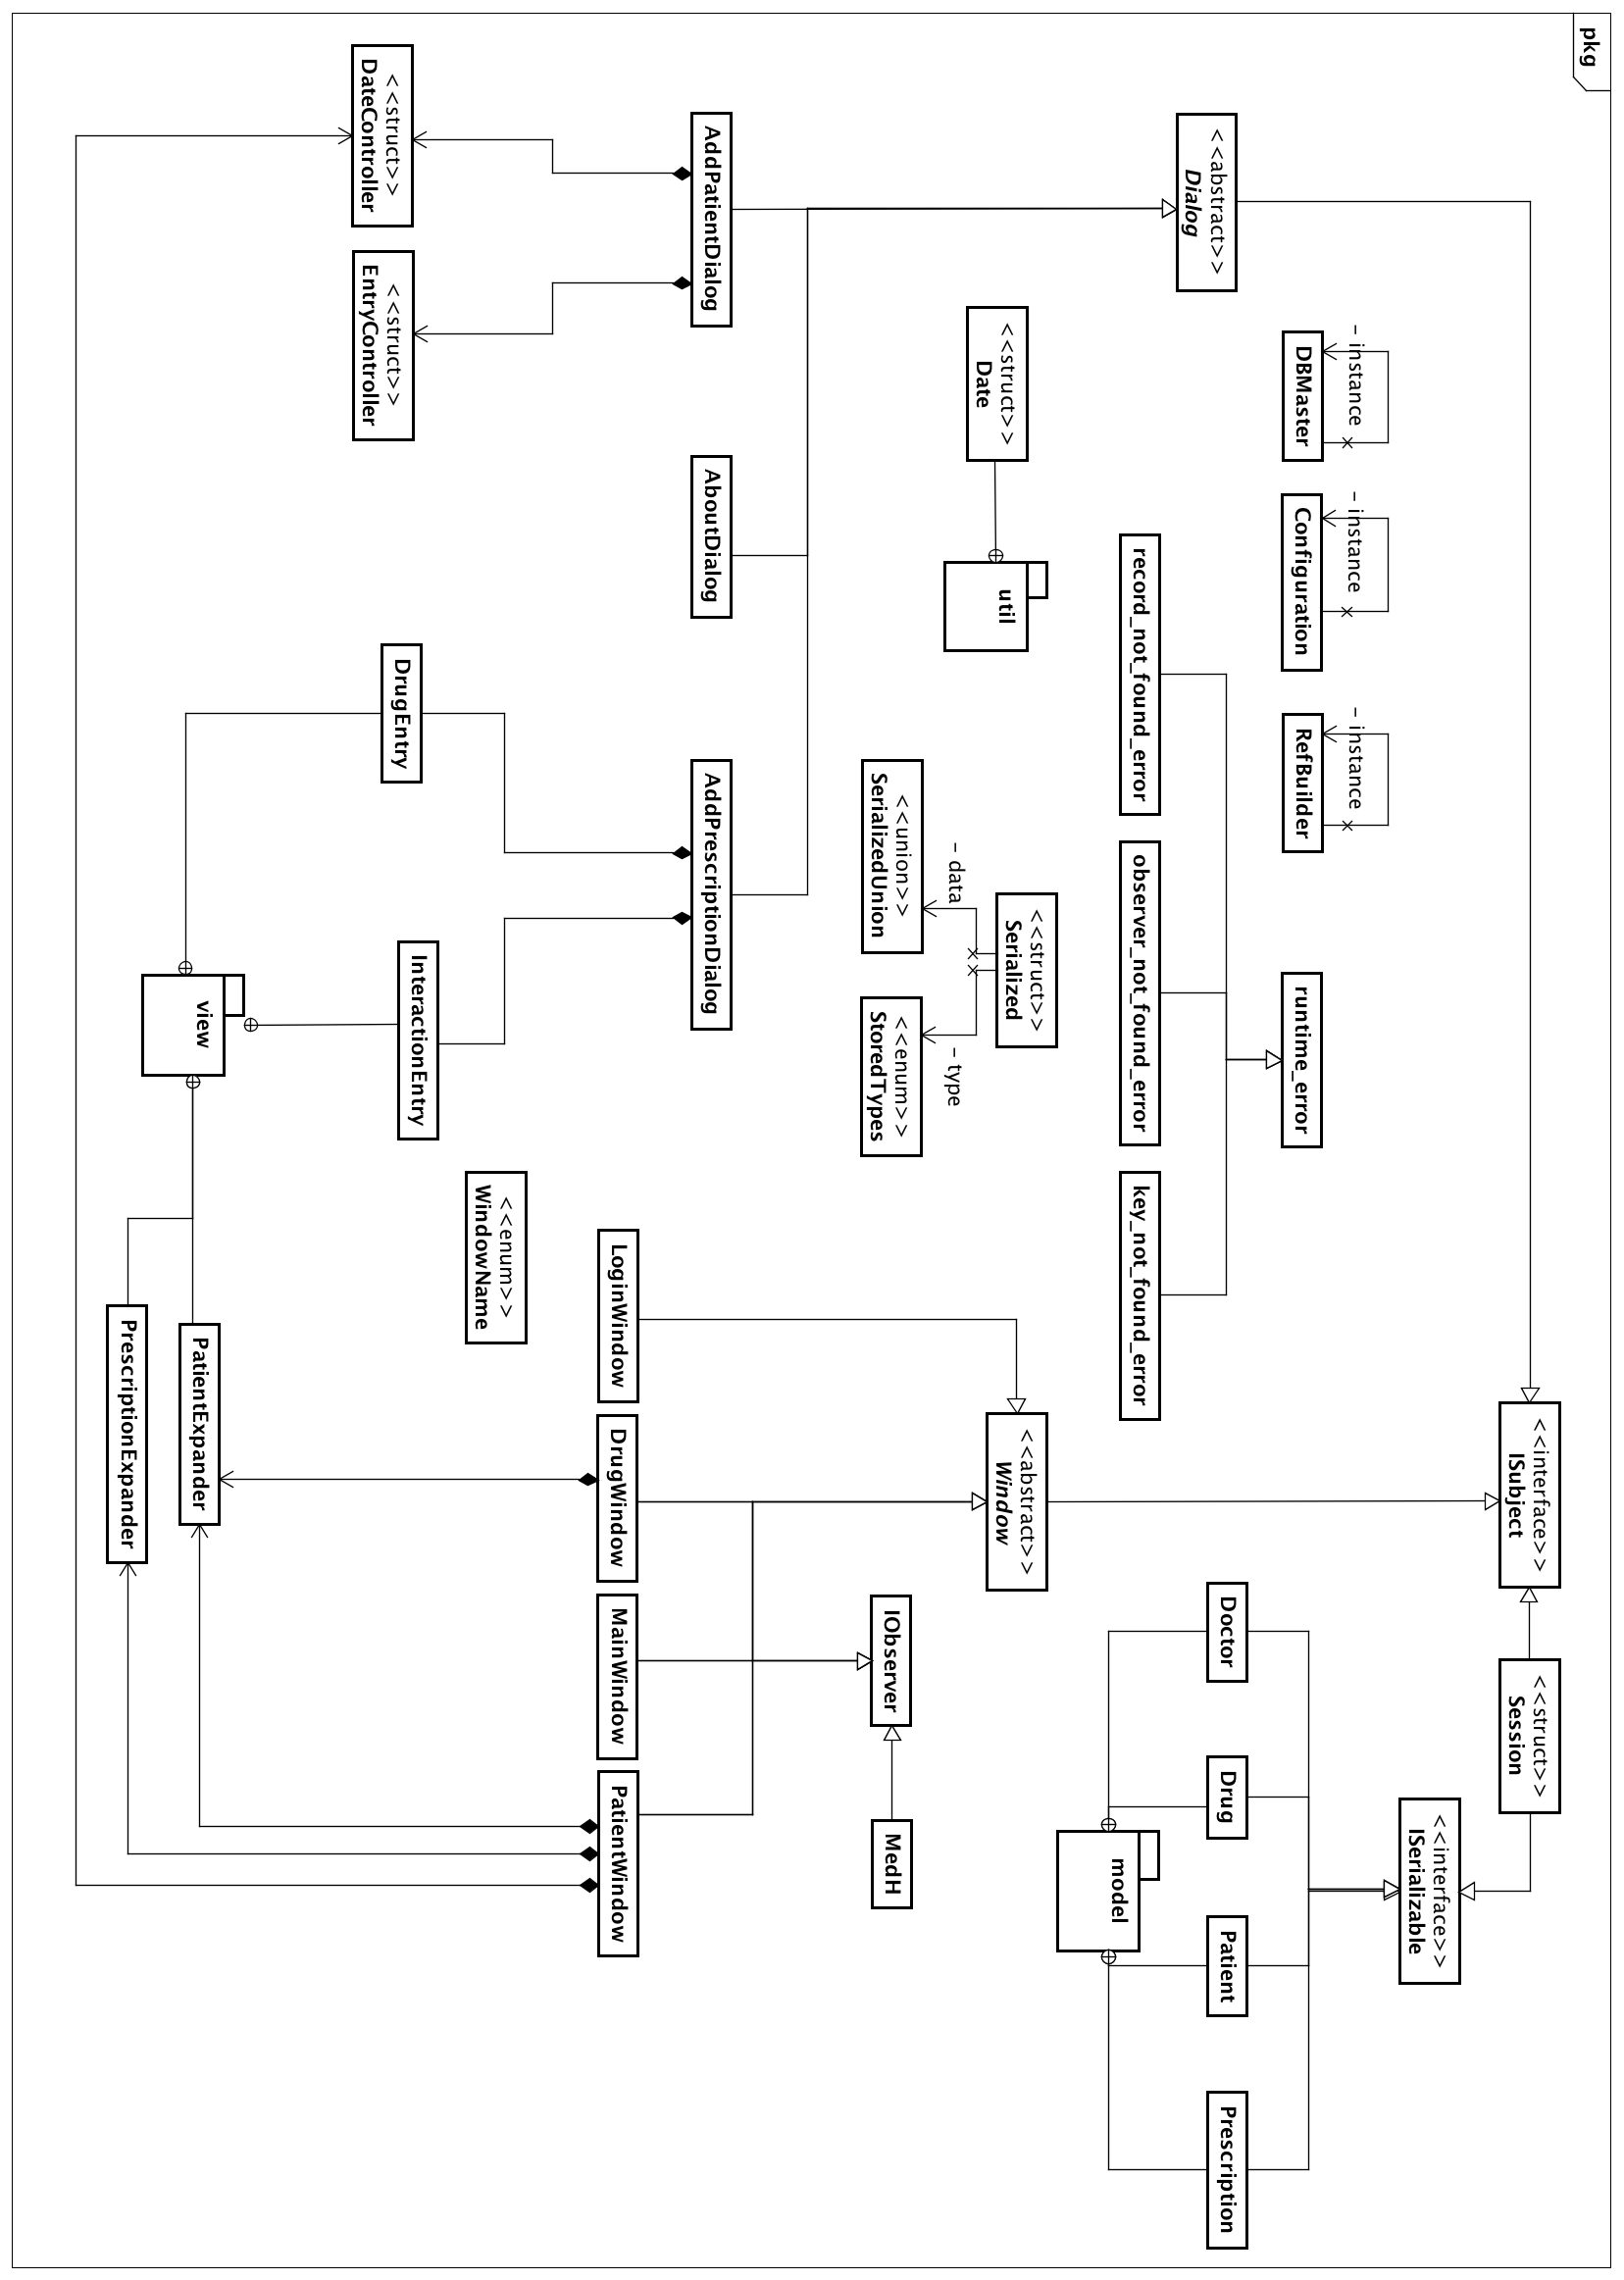
\includegraphics[width=0.9\textwidth,keepaspectratio]{Class_diagram_min.png}
\end{figure}

\newpage
\subsection{Sequence Diagram}
\safeImage{Inserimento_paziente_seq.png}
\safeImage{Visualizza_prescrizioni_filtrate_seq.png}
\safeImage{Login_sequence_seq.png}

\section{Scelte Progettuali}
Why:
Linguaggio
Glade - css
Gtkmm3
Configurazione
Database (banale)
Motivazioni della gui
Github - sviluppo semiagile


\subsection{MVC Pattern}
Due parole mvc, immagine di intercomunicazione

View in xml

Custom view in classi

Controller classi

Model classi

\subsection{Singleton Pattern}
Globali sulle classi

Sono lazy -> differenza

DBMaster

Configuration

RefBuilder

\subsection{Observer Pattern}
Adattato al modello
Usato coi dialog -> comodo per gli update asincroni e differenziati

\section{Conclusioni}
È un prototipo - manca di funzionalità

Vantaggi prototipo:
- interfacciamento easy

Vantaggi codice:
- facilmente adattabile (estensibile)

Schifi:
- scelta della libreria grafica pessima -> sarebbe stato meglio qt
- non siamo capaci di dare i nomi alle cose
- ridondanza nel codice



\end{document}
